\documentclass[a4paper]{article}
\usepackage{fancyvrb}
\usepackage{color}

\author{Emmanuel Paradis}
\title{A Little Sweave Document}

\usepackage{Sweave}
\begin{document}

\maketitle

\section{Introduction}

This small document can be used as a Sweave template. It
uses minimal formatting of the text.

You can use Sweave with very little knowledge of LaTeX, but the
presentation of the text will be a little crude. Anyway, we have used
`author' and `title' that define these items before the document
begins. The command `maketitle' prints this information together with
the current data. Finally the command `section' defines numbered
sections within the text. All these commands are case-sensitive. That
will be all about LaTeX for the moment (but you may have noticed that
opening single quote is specified with a backquote... ;) ).

You know that R codes in a Sweave document starts with `< < > > =' and
ends with `@'. This last character should be followed either by a
white space, or by blank line (or both). Let's try it with some random data:

\begin{Schunk}
\begin{Sinput}
> x <- rnorm(1000)
> x[1:10]
\end{Sinput}
\begin{Soutput}
 [1] -0.24555704  0.94196672 -0.68219638  1.10484918 -0.10652145  0.03923254  0.44805955  0.32163824  1.07459930
[10]  0.34391869
\end{Soutput}
\end{Schunk}

Both input and output are printed. Suppose we want only the output:

\begin{Schunk}
\begin{Soutput}
 [1] -1.0478118  0.3942632  1.3823847 -0.2940653 -0.7029665 -2.4368603 -0.3751244  1.9271871  0.9044205
[10]  1.8291364
\end{Soutput}
\begin{Soutput}
[1] "airquality" "islands"    "x"          "y"          "z"         
\end{Soutput}
\end{Schunk}

The options are specified within the `< < > > =' starting the R chunk. A
related option is `quiet=true' which suppresses the input, so some R
commands can be executed silently:


Let's check that it has run with a normal R chunck:

\begin{Schunk}
\begin{Sinput}
> ls()
\end{Sinput}
\begin{Soutput}
[1] "airquality" "islands"    "x"          "y"          "z"         
\end{Soutput}
\end{Schunk}

\section{Including Figures}

To have a plot included, we must add the option `fig=true' in the R
chunck header:

\begin{Schunk}
\begin{Sinput}
> hist(x)
\end{Sinput}
\end{Schunk}
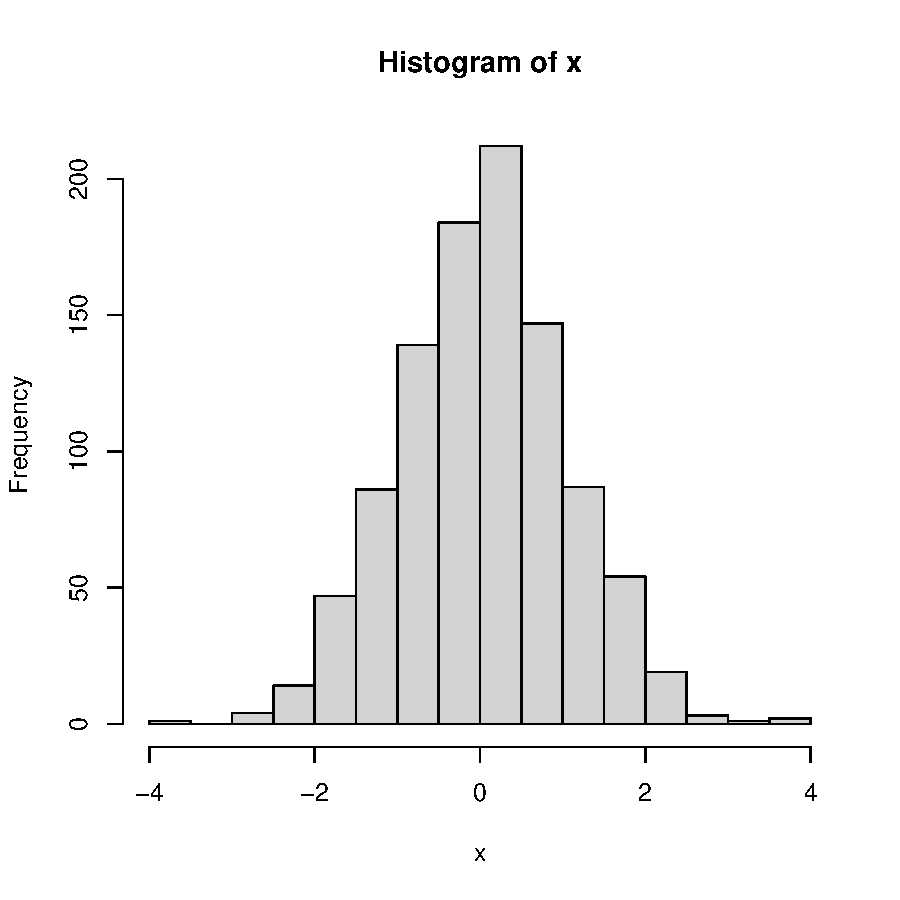
\includegraphics{Little_Sweave-005}

This will create two files in the working directory: a PDF version of
the plot, and an EPS one. The names of these files are created
automatically by Sweave. In case you don't know what is your R working directory:

\begin{Schunk}
\begin{Sinput}
> getwd()
\end{Sinput}
\begin{Soutput}
[1] "/Users/marguerite/Library/Mobile Documents/com~apple~CloudDocs/Documents/git/rclass-2025/posts/2025-01-28-intro-quarto"
\end{Soutput}
\end{Schunk}

If you want to make many plots, it's useful to work in a distinct (sub)directory.

You can't really have several plot commands within the same R chunck,
but you can use `layout' to make several plots on the same figures:

\begin{Schunk}
\begin{Sinput}
> layout(matrix(c(1, 2, 1, 3), 2))
> plot(x, y)
> hist(x)
> hist(y)
\end{Sinput}
\end{Schunk}
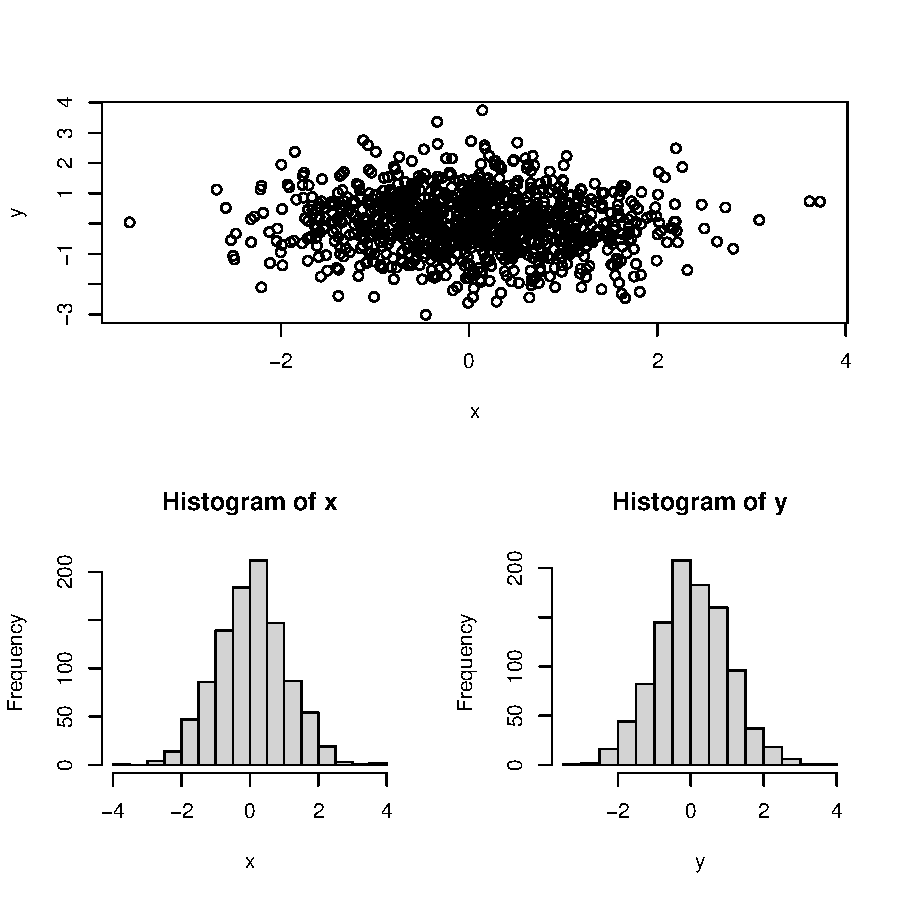
\includegraphics{Little_Sweave-007}

Any R command can be put in the R chuncks. Let's check out the islands built-in dataset, it contains areas of the worlds islands in thousands of square miles:

\begin{Schunk}
\begin{Sinput}
> data(islands)
> dotchart(log(islands[order(islands)], 10),
+    main = "islands data: log10(area) (log10(sq. miles))")
\end{Sinput}
\end{Schunk}
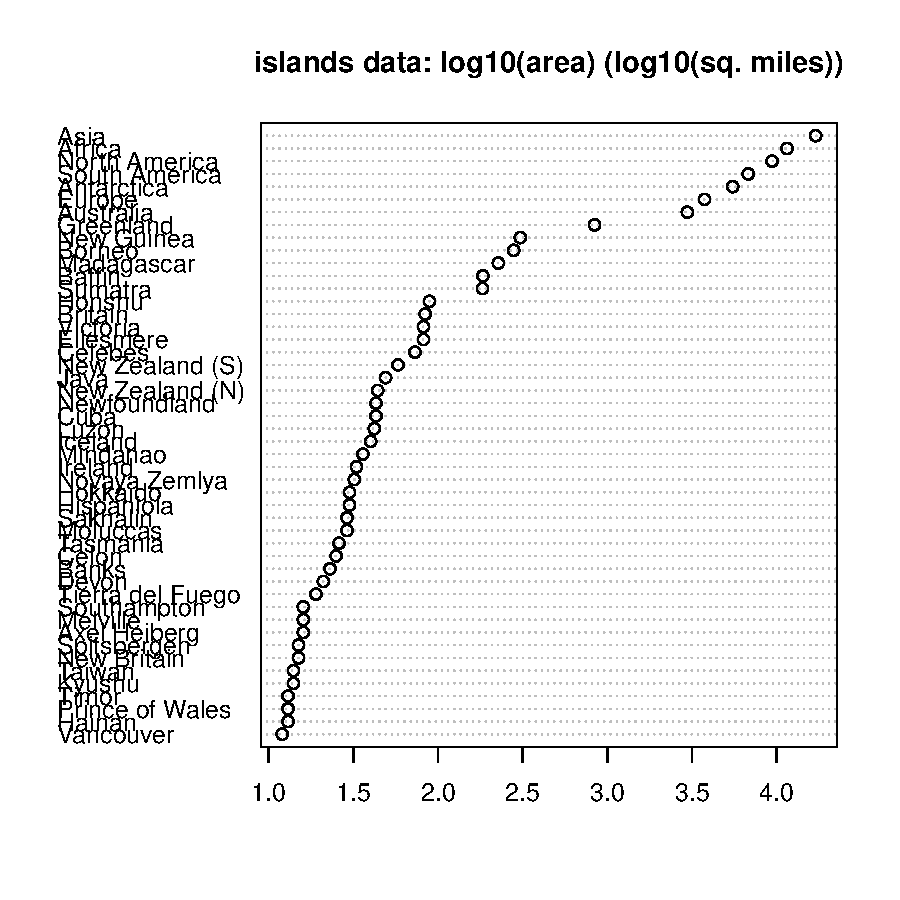
\includegraphics{Little_Sweave-008}

The nice thing with Sweave is that you know exactly which data file
has been used since the code has been executed at the same time than
the document is printed!

\section{Conclusion}

I hope this starter will give you the feel to write many Sweave
documents. A final word about LaTeX:	it
ignores  		 		 		 		 		 		 		 		 		 		 		 		 		 		 		 		 		 		 		 		 		 		 		 		 		 		 		 		 		 		extra
white  		 		 		 		 		 		 		 		 		 		 		 		 		 		 		spaces
 		 		 		 		 		 		 		 		 		 		between
words.

\end{document}
